\section{Measurement Routine}
\label{sec:routine}

The routine is written in Python.
This brings in several advantages:
First of all we can actually look through the code
and comment on it,
where clarification is needed.
The Python syntax is simple enough --
basically, English with peculiar grammar --
so if you can read this documentation,
you will understand the program just as well.
LabView for example
fails at exactly this point;
it's very hard to maintain,
and the different sections
of the script are difficult to interpret
(let alone the litteral spaghetti code).
And lastly,
with Python we don't depend on a third party license.
Again, LabView and Matlab
fail at this point.

\subsection{The routine}
\label{sec:routine:routine}

You either look at the example
given in ``exp/eval/routine\_measurement.py''
and read it through,
or you continue to read here.
The following long text covers the same.

We choose a set of values corresponding to
a) the current of the pump laser,
and b) the temperatures of the heat sink.
We specify further, a path where to store the results.
And lastly, we choose on how often every power current
is ought to be measured --
repeated measurements in order to obtain
the errorbars
that inform us on the reliability of the results.

At each temperature,
we set the power source to the requested currents,
and read out the power meters.
The results of each power meter is written in its own file.
Each of these files starts with a header line,
that contains the state of the relevant settings of the device in question.
Consequentially,
if we doubt the integrity of the measurements
we can look at this header line and
at least know what state the device has reported to be in.
The information about the power source
are also written to its own file,
containing the set and actual current.
Hence, at each temperature we generate
one file for the power source, plus one for each power meter.

At the end of these measurements we write a line in a logfile:
The set temperature,
the actually reached temperature,
the filenames of the files
with the results of the different devices,
along with a timestamp so we know which measurement took how long.
The timestamp also allows us to connect certain effects
to the time of the day it was measured.
The approach with a logfile
and the separate files of each device
(whose names are automatically stored in the logfile),
facilitates the analysis;
all the information a analysis-script needs is specified in the logfile.

At each heat sink temperature
we irradiate the sample
with different pump powers.
Each pump is repeated $N$ times over all.
The pump order is selected at random,
as illustrated in Fig.~\ref{img:random_sampling}.
Thanks to the random sampling
the measurement results
are detached from the lab environment --
most notably time-independent.
The heat sink cannot control its temperature
with absolute precision.
Figure~\ref{img:random_sampling_heatsink}
illustrates this issue:
It shows
the actually present heat sink temperature
for six set temperatures.
In the left column
the temperatures are plotted
in chronological order.
We can identify,
the temperature drifts.
The right column shows the same temperatures,
but corresponding to the set pump.
The repeated measurements
see a spread of different temperatures
but the temporal drifts can not be resolved.

In contrast,
Fig.~\ref{img:random_sampling_ramp_heatsink}
shows the heat sink temperature
during a measurement without the random pump selection.
In this case, clearly,
we cannot talk about a single heat sink temperature
for all the pump settings
for this specific set heat sink temperature.
The resulting measurements are highly repeatable,
but only given the same pump order.
This pseudo-stability
we exploit
during the calibration process
of the different beam samplers
and detectors:
During the calibration
we don't care about reproducibility
but solely about the repeatability
of two consecutive measurements.

\begin{figure}
\centering
\subfigure{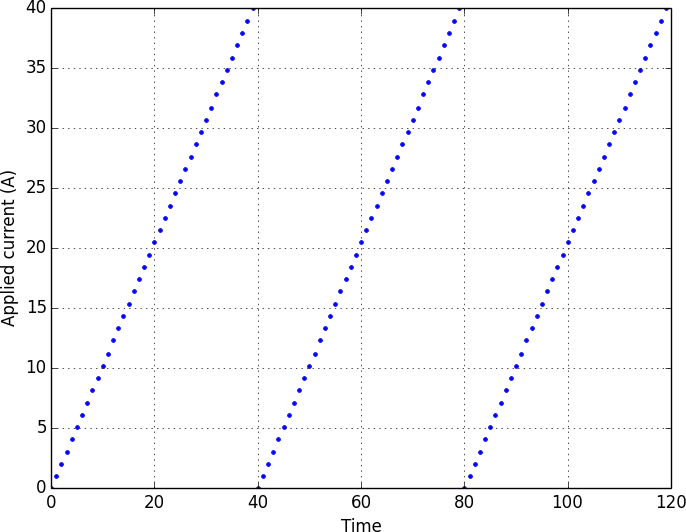
\includegraphics[width=7cm]{img/random_sampling_ramp.png}}
\subfigure{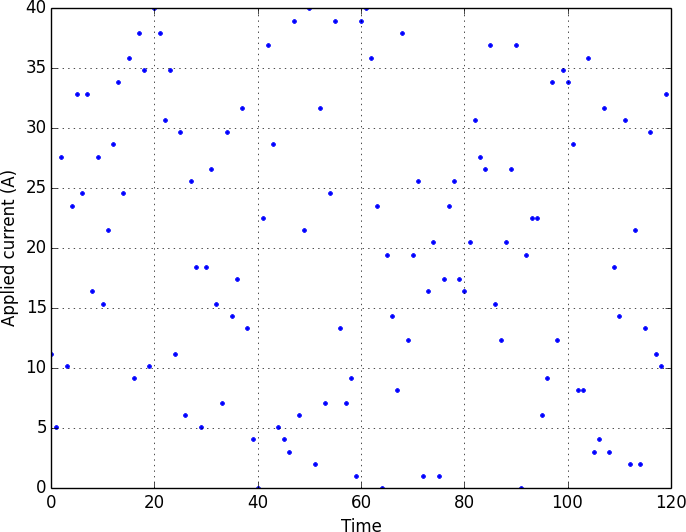
\includegraphics[width=7cm]{img/random_sampling_random.png}}
\caption{Two examples to apply various pump settings, with a repetition rate of 3.
Left: A ramp. Right: Random sampling.}
\label{img:random_sampling}
\end{figure}

\begin{figure}
\centering
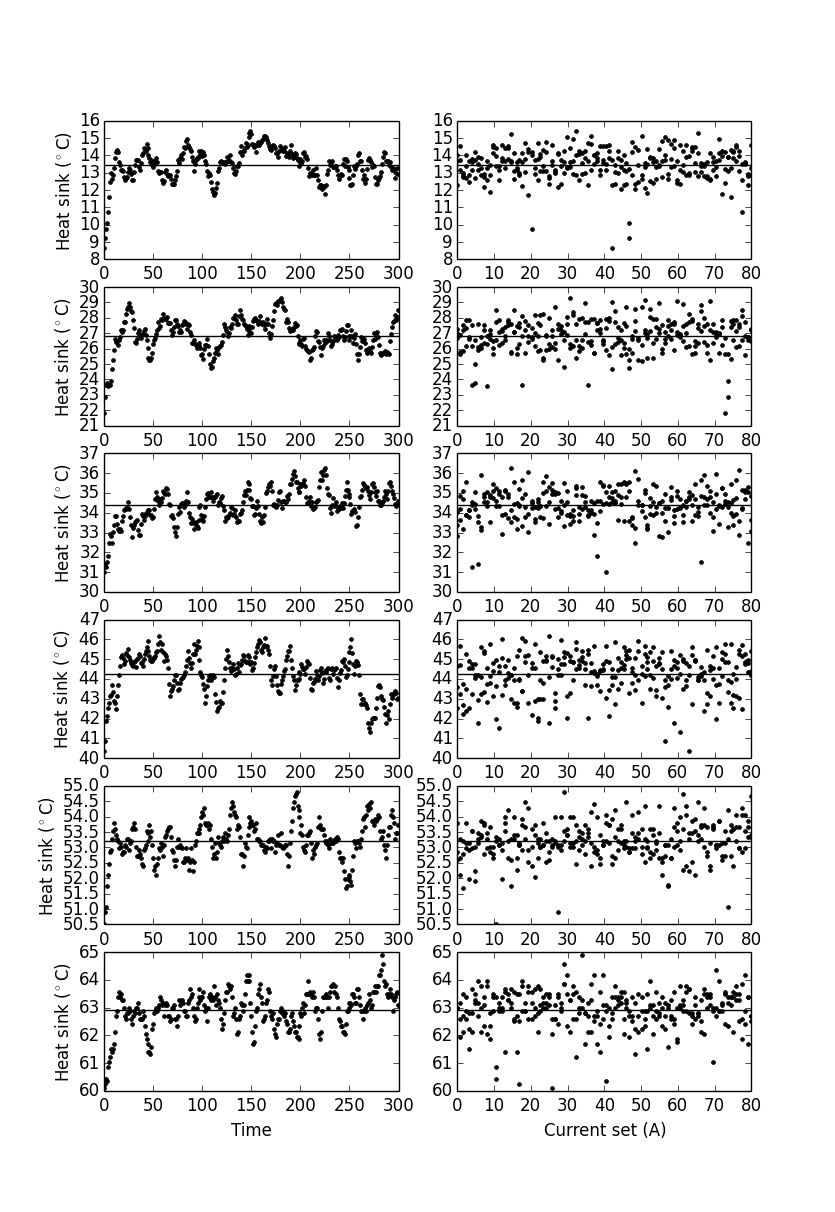
\includegraphics[width=15cm]{img/random_sampling_heatsink.png}
\caption{The heat sink temperature fluctuates over time (left).
Thanks to the random sampling addressed in Fig.~\ref{img:random_sampling}
the measurements don't see these drifts (right).}
\label{img:random_sampling_heatsink}
\end{figure}

\begin{figure}
\centering
\subfigure{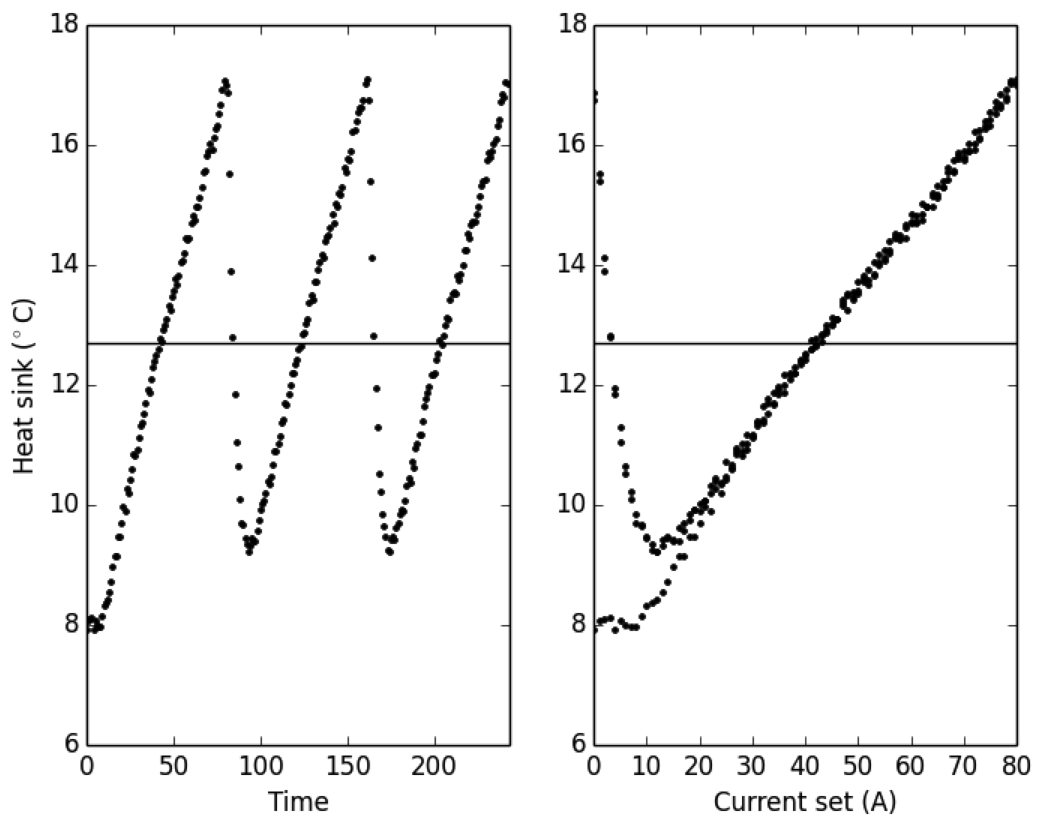
\includegraphics[width=7cm]{img/random_sampling_ramp_heatsink.png}}
\subfigure{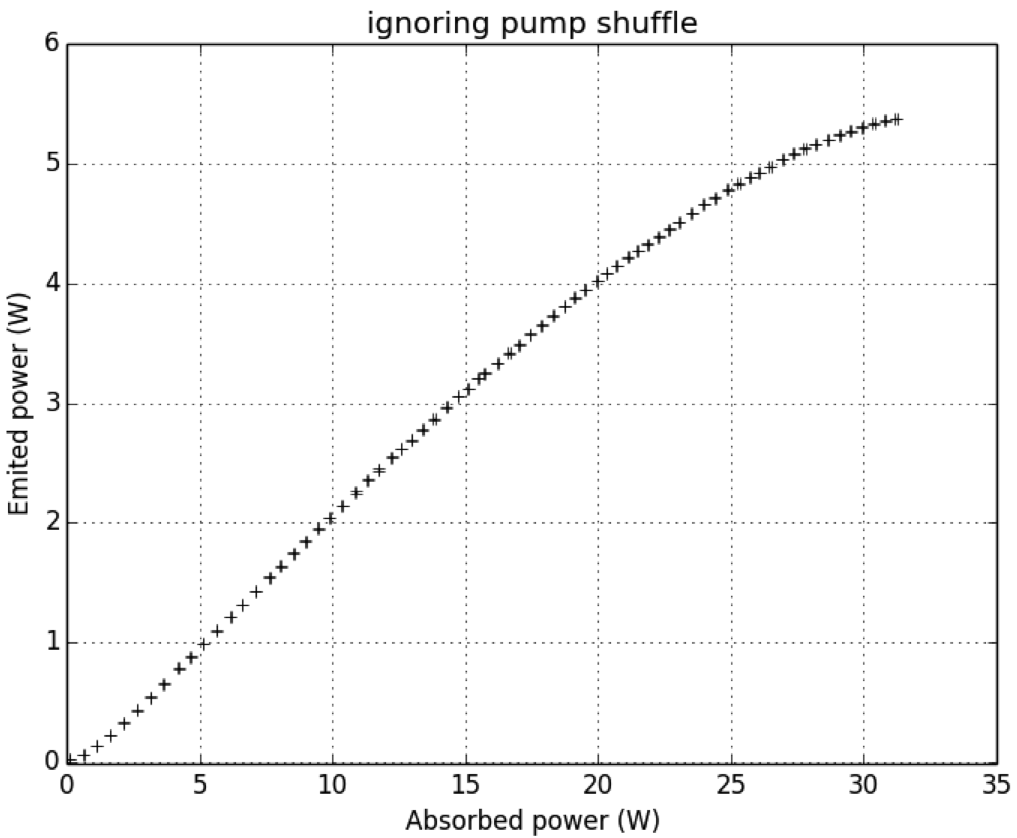
\includegraphics[width=7cm]{img/random_sampling_ramp_noisfreeLL.png}}
\caption{In contrast to Fig.~\ref{img:random_sampling_heatsink},
when we ignore the random pump sampling
highlighted in Fig.~\ref{img:random_sampling},
the temperature seen by the single pump settings
differ strongly from the average heat sink temperature
(left).
The resulting LL-characteristic
has very little noise on its data points
(right).
But these small error bars dismiss the fact
that the underlying points were measured
under very different conditions;
eroding the significance
of this low noise.}
\label{img:random_sampling_ramp_heatsink}
\end{figure}

The power meter average each measurement point
over 200 samples,
of which each one sample
takes approx. 3 ms \cite{ThorlabsPM}.

The order of heat sink temperature
is still a ramp:
I expect the setting of a new temperature to be somewhat time consuming.
Therefore, we want to make use of the previously set temperature.
The measurement routine looks at the specified temperature range,
picks the one closest to room temperature,
and increases to every second entry.
Once the highest temperature is reached,
the residual temperatures are picked,
in descending order, until the lowest temperature is reached.
From there we heat back up to room temperature.
This routine is illustrated in Fig.~\ref{img:temproutine}.

\begin{figure}
\centering
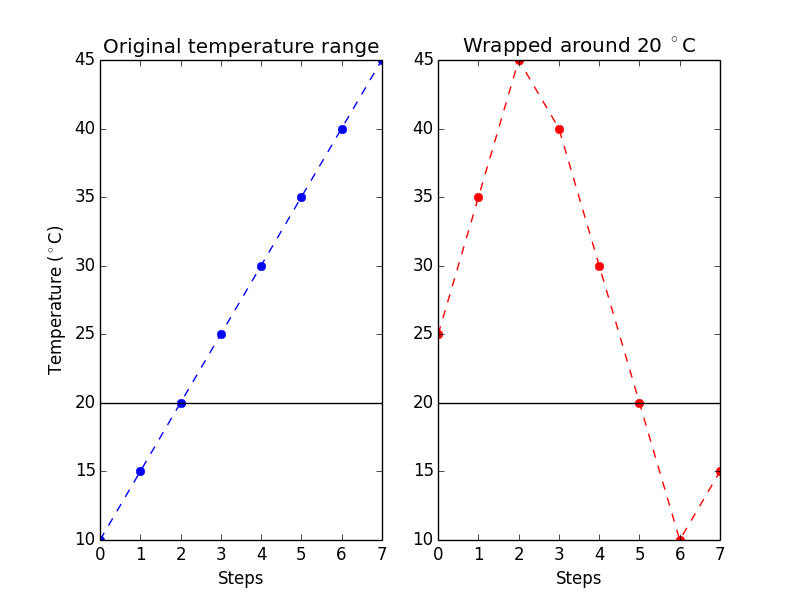
\includegraphics[width=12.5cm]{img/temp_wrap.png}
\caption{An example of how a given temperature range is wrapped around the room temperature
(here assumed to be \degr{20}).}
\label{img:temproutine}
\end{figure}

As mentioned already,
we repeated the measurement of each pump setting
$N$ times.
With this repetition we obtain a measure
for how well we know
the underlying true value.
We are hence interested in
the mean of these single measurements and
the resulting unbiased standard error \cite{Barlow}
\begin{equation}
\Delta x = \sqrt{ \frac{1}{N(N-1)}
	\sum\limits_{i=1}^N (x_i - 
		\frac{1}{N} \sum\limits_{i=1}^N x_i )^2 }.
\label{eq:sterr}
\end{equation}

For the uncertainties attached to
quantities obtained through fits,
I use a so-called
Jackknife \cite{Efron1983} approach:
In a nutshell,
this method allows to estimate
the influence of the single measurement points
on the fit parameters
without working through
the covariance matrix of the fit.
The resulting error value
is directly related with the
unbiased standard error (\ref{eq:sterr}),
used for the rest of the report.

\subsection{Safety precautions}
\label{sec:routine:safety}

The goal of this script is to automate as much as possible.
Ideally,
we want to install a new VECSEL,
align the output coupler,
press start,
and return some time later to a complete data set
for this specific VECSEL under test.
For this we need to be sure
our measurement routine handles potential errors appropriately.

For this we must not rely on software.
Instead, we have to implement the safety precautions on hardware side.
In software we can try to mitigate
potential problems through proper error handling.
I don't know how this would be done in LabView.
In Matlab and Python this is performed through so-called
try/catch and try/except handles, respectively.
With it I have implemented that if anything goes wrong software side,
the power source is shut down
(This order itself is so low-level,
that it \textit{should} always work.).
For example, one of the devices could send an unexpected answer,
the heat sink doesn't reach its requested temperature within reasonable time, etc.
For the unlikely event
that even the power source shut down doesn't work,
we have to implement the safety precautions on hardware side.

Our power source has two ways to be shut down:
We can disable the current,
or we can set the current to zero.
In order to disable the current,
we first have to ask the power source,
whether the current is currently applied.
If it is, we toggle it like a light-switch to shut off.
However, querying the current state
is error-prone.
Hence, if an error is caught we leave the shutter to be in what ever state it is
and only set the current to zero.
Potentially it is still applied.
But the light output at $0\,\mathrm{A}$
is barely detectable --
but there still \emph{is} a leak flow of photons.
Writing to the power source should not cause any new problems,
so simply writing $0\,\mathrm{A}$ should go through.

On the hardware side,
the ``laser on'' light in front of the lab
is controlled by a logic tied to the power source:
As soon as the power source applies a certain specified voltage
the laser warning turns on.
During the measurements this safety sign therefore
is always on.

As a second safety precaution I supply a script that allows us to test 
modifications on the measurement routine with fake devices.
In order to connect the measurement routine with the measurement devices
we have to specify a protocol.
In the new script we do this by selecting an external file
that contains the initiation details.
By specifying the fake protocol we can modify the routine without the real devices.
This separation in code is, for one, good practice,
and secondly convenient if we cannot use one of the devices due to a revision or whatever.
To be detached from the physical devices was not possible with the old script --
which is one of the reasons why it was possible to toggle the power source shutter
while setting the wavelength of the power meter.

